%% LyX 1.3 created this file.  For more info, see http://www.lyx.org/.
%% Do not edit unless you really know what you are doing.
%\documentclass[letterpaper,twocolumn,english]{article}
%\usepackage[T1]{fontenc}
%\usepackage[latin1]{inputenc}
%\usepackage{graphicx}

%\makeatletter

\documentclass[letterpaper,twocolumn,english]{article}
\usepackage[latin1]{inputenc}
\usepackage{graphicx}
\usepackage{usenix,epsfig}


%%%%%%%%%%%%%%%%%%%%%%%%%%%%%% LyX specific LaTeX commands.
%% Bold symbol macro for standard LaTeX users
%\newcommand{\boldsymbol}[1]{\mbox{\boldmath $#1$}}


%%%%%%%%%%%%%%%%%%%%%%%%%%%%%% User specified LaTeX commands.
\usepackage[T1]{fontenc}
\usepackage{ae,aecompl}

%\usepackage{babel}
%\makeatother

\begin{document}

\date{}

\title{\Large \bf LLADD: Extensible Transactional Storage FIXME}

\author{
Your N.\ Here \\
%{\em Your Department} \\
{\em Your Institution}\\
%{\em Your City, State, ZIP}\\
% is there a standard format for email/URLs??
% remember that ~ doesn't do what you expect, use \~{}.
{\normalsize yourname@host.site.dom, http://host.site.dom/yoururl} \\
%
% copy the following lines to add more authors
 \smallskip
 Name Two Here \\
{\em Two's Institution}\\
%% is there a standard format for email/URLs??
{\normalsize two@host.site.dom, http://host.site.dom/twourl}
%
} % end author

\maketitle

\thispagestyle{empty}

\subsection*{Abstract}

Although many systems provide transactionally consistent data management,
existing implementations are generally monolithic and tied to a higher-level DBMS, limiting the scope of their usefulness to a single application,
or a specific type of problem. As a result, many systems are forced
to ``work around'' the data models provided by a transactional storage
layer. Manifestation of this problem include 'impedence mismatch'
in the database world and the limited number of data models provided
by existing libraries such as BerkeleyDB. In this paper, we describe
a light-weight, easily extensible library, LLADD, that allows application
developers to develop scalable and transactional application-specific
data structures. We demonstrate that LLADD is simpler than prior systems
and is very flexible, while performing favorably in a number of
micro-benchmarks. We also describe, in simple and concrete terms,
the issues inherent in the design and implementation of robust, scalable
transactional data structures. In addition to the source code, we
have also made a comprehensive suite of unit-tests, API documentation,
and debugging mechanisms publicly available.%
\footnote{http://lladd.sourceforge.net/%
}


\section{Introduction}

Changes in data models, consistency requirements, system scalibility,
communication models and fault models require changes to the storage
and recovery subsystems of modern applications. 

For applications that are willing to store all of their data in a
DBMS, and access it only via SQL, existing databases are just fine and
LLADD has little to offer.  However, for those applications that need
more direct management of data, LLADD offers a layered architecture
that enables simple but robust data management.\footnote{Such
applications are ``navigational'' in the database vocabulary, as they
directly navigate data structures rather than perform set operations.}

The basic approach of LLADD, taken from ARIES [xx], is to build
\emph{transactional pages}, which enables recovery on a page-by-page
basis, despite support for high concurrency and the minimization of
seeks during commit (by using a log).  We show how to build a variety
of useful data managers on top of this layer, including persistent
hash tables, lightweight recoverable virtual memory, and simple
databases.  We also cover the details of crash recovery,
application-level support for transaction abort and commit, and basic
latching for multithreaded applications.

[more coverage of kinds of apps?  imap, lrvm, cht, file system, database]

Many implementations of transactional pages exist in industry and
in the literature. Unfortunately, these algorithms tend either to
be straightforward and unsuitable for real-world deployment, or are
robust and scalable, but achieve these properties by relying upon
intricate sets of internal (and often implicit) interactions. The
ARIES algorithm falls into the second category, has been extremely
sucessful as part of the IBM DB2 database system.
It provides performance and reliability that is comparable to that of current
commercial and open-source products. Unfortunately, while the algorithm
is conceptually simple, many subtlties arise in its implementation.
We chose ARIES as the basis of LLADD, and have made a significant
effort to document these interactions. Although  a complete discussion
of the AIRES algorithm is beyond the scope of this paper, we will
provide a breif overview, and explain the details that are relevant
to developers that wish to extend LLADD. 

By documenting the interface between AIRES and higher-level primitives
such as data structures, and by structuring LLADD to make this
interface explicit in both the library and its extensions, we hope to
make it easy to produce correct and efficient durable data
structures. In existing systems (and indeed, in earlier versions of
LLADD), the implementation of such structures is extremely
complicated, and subject to the introduction of incredibly subtle
errors that would only be evident during crash recovery or at other
inconvenient times.  Thus there is great value is reusing these lower
layers once developed.

Finally, by approaching this problem by implementing a number of simple
modules that ``do one thing and do it well'', we believe that
LLADD can provide competitive performance while making future improvements
to its core implementation significantly easier. In order to achieve
this goal, LLADD has been split into a number of modules forming a
'core library', and a number of extensions called 'operations' that
build upon the core library. Since each of these modules exports a
stable interface, they can be independently improved.


\subsection{Prior Work\label{sub:Prior-Work}}

An extensive amount of prior work covers the algorithms presented in
this paper.  Most fundamentally, systems that provide transactional
consistency to their users generally include a number of common
modules.  A high-level overview of a typical system is given in Figure
\ref{cap:DB-Architecture}.  

\begin{figure}
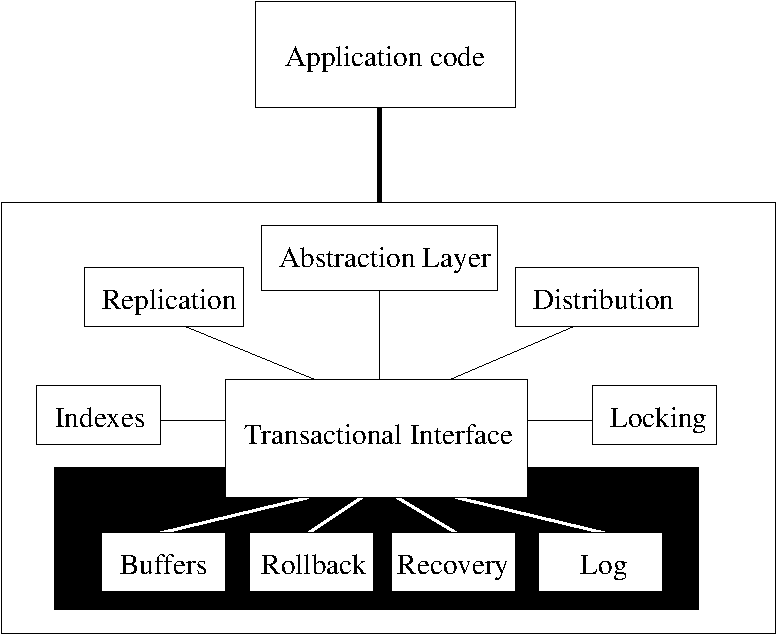
\includegraphics[%
  width=1.0\columnwidth]{DB-Architecture.pdf}


\caption{\label{cap:DB-Architecture}Conceptual view of a modern
transactional application.  Current systems include high level
functionality, such as indices and locking, but are not designed to
allow developers to replace this functionality with application
specific modules.}
\end{figure}

Many applications make use of transactional storage, and each is
designed for a specific application, or set of applications.  LLADD
provides a flexible substrate that allows such applications to be
developed.  The complexity of existing systems varies widely, as do
the applications for which these systems are designed.  

On the database side of things, relational databases excel in areas
where performance is important, but where the consistency and
durability of the data is crucial.  Often, databases significantly
outlive the software that uses them, and must be able to cope with
changes in business practices, system architechtures, etc.

Object-oriented databases are more focused on facilitating the
development of complex applications that require reliable storage, but
may take advantage of less-flexible, but more efficient data models,
as they often only interact with a single application, or a handful of
variants of that application.

Databases are designed for circumstances where development time may
dominate cost, many users must share access to the same data, and
where security, scalability, and a host of other concerns are
important.  In many, if not most circumstances, these issues are less
important, or even irrelevant.  Therefore, applying a database in
these situations is likely overkill, which may partially explain the
popularity of MySQL, which allows some of these constraints to be
relaxed at the discretion of a developer or end user.

Still, there are many applications where MySQL is still too
inflexible.  In order to serve these applications, a host of software
solutions have been devised.  Some are extremely complex, such as
semantic file systems, where the file system understands the contents
of the files that it contains, and is able to provide services such as
rapid search, or file-type specific operations such as thumbnailing,
automatic content updates, and so on.  Others are simpler, such as
BerkeleyDB, which provides transactional storage of data in unindexed
form, in indexed form using a hash table, or a tree.  LRVM, a version
of malloc() that provides transacational memory, and is similar to an
object oriented database, but is much lighter weight, and more
flexible.

Finally, some applications require incredibly simple, but extremely
scalable storage mechanisms.  Cluster Hash Tables are a good example
of the type of system that serves these applications well, due to
their relative simplicity, and extremely good scalability
characteristics.  Depending on the fault model a cluster hash table is
implemented on top of, it is also quite plasible that key portions of
the transactional mechanism, such as forcing log entries to disk, will
be replaced with other durability schemes, such as in-memory
replication across many nodes, or multiplexing log entries across
multiple systems.  This level of flexibility would be difficult to
retrofit into existing transactional applications, but is appropriate
in many environments.

We have only provided a small sampling of the many applications that
make use of transactional storage.  Unfortunately, it is extremely
difficult to implement a correct, efficient and scalable transactional
data store, and we know of no library that provides low level access
to the primatives of such a durability algorithm.  These algorithms
have a reputation of being complex, with many intricate interactions,
which prevent them from being implemented in a modular, easily
understandable, and extensible way.  In addition to describing such an
implementation of ARIES, a popular and well-tested
'industrial-strength' algorithm for transactional storage, this paper
will outline the most important interactions that we discovered (that
is, the ones that could not be encapsulated within our
implementation), and give the reader a sense of how to use the
primatives the library provides.



%Many plausible lock managers, can do any one you want.

%too much implemented part of DB; need more 'flexible' substrate.



\section{ARIES from an Operation's Perspective}

Instead of providing a comprehensive discussion of ARIES, we will
focus upon those features of the algorithm that are most relevant
to a developer attempting to add a new set of operations. Correctly
implementing such extensions is complicated by concerns regarding
concurrency, recovery, and the possibility that any operation may
be rolled back at runtime.

We first sketch the constraints placed upon operation implementations,
and then describe the properties of our implementation of ARIES that
make these constraints necessary. Because comprehensive discussions
of write ahead logging protocols and ARIES are available elsewhere,
(Section \ref{sub:Prior-Work}) we only discuss those details relevant
to the implementation of new operations in LLADD.


\subsection{Properties of an Operation\label{sub:OperationProperties}}

A LLADD operation consists of some code that performs some action
on the developer's behalf. These operations implement the actions
that are composed into transactions. Since transactions may be aborted,
the effects of an operation must be reversible. Furthermore, aborting
and comitting transactions may be interleaved, and LLADD does not
allow cascading abort,%
\footnote{That is, by aborting, one transaction may not cause other transactions
to abort. To understand why operation implementors must worry about
this, imagine that transaction A split a node in a tree, transaction
B added some data to the node that A just created, and then A aborted.
When A was undone, what would become of the data that B inserted?%
} so in order to implement an operation, we must implement some sort
of locking, or other concurrency mechanism that protects transactions
from each other. LLADD only provides physical consistency; we leave
it to the application to decide what sort of transaction isolation is appropriate.
Therefore, data dependencies between transactions are allowed, but
we still must ensure the physical consistency of our data structures.

Also, all actions performed by a transaction that commited must be
restored in the case of a crash, and all actions performed by aborting
transactions must be undone. In order for LLADD to arrange for this
to happen at recovery, operations must produce log entries that contain
all information necessary for undo and redo.

Finally, each page contains some metadata needed for recovery. This
must be updated apropriately.


\subsection{Normal Processing}


\subsubsection{The buffer manager}

LLADD manages memory on behalf of the application and prevents pages
from being stolen prematurely. While LLADD uses the STEAL policy and
may write buffer pages to disk before transaction commit, it still
must make sure that the redo and undo log entries have been forced
to disk before the page is written to disk. Therefore, operations
must inform the buffer manager when they write to a page, and update
the log sequence number of the page. This is handled automatically
by many of the write methods provided to operation implementors (such
as writeRecord()), but the low-level page manipulation calls (which
allow byte level page manipulation) leave it to their callers to update
the page metadata appropriately.


\subsubsection{Log entries and forward operation (the Tupdate() function)\label{sub:Tupdate}}

In order to handle crashes correctly, and in order to the undo the
effects of aborted transactions, LLADD provides operation implementors
with a mechanism to log undo and redo information for their actions.
This takes the form of the log entry interface, which works as follows.
Operations consist of a wrapper function that performs some pre-calculations
and perhaps acquires latches. The wrapper function then passes a log
entry to LLADD. LLADD passes this entry to the logger, and then processes
it as though it were redoing the action during recovery, calling a function
that the operation implementor registered with
LLADD. When the function returns, control is passed back to the wrapper
function, which performs any post processing (such as generating return
values), and releases any latches that it acquired. %
\begin{figure}
~~~~~~~~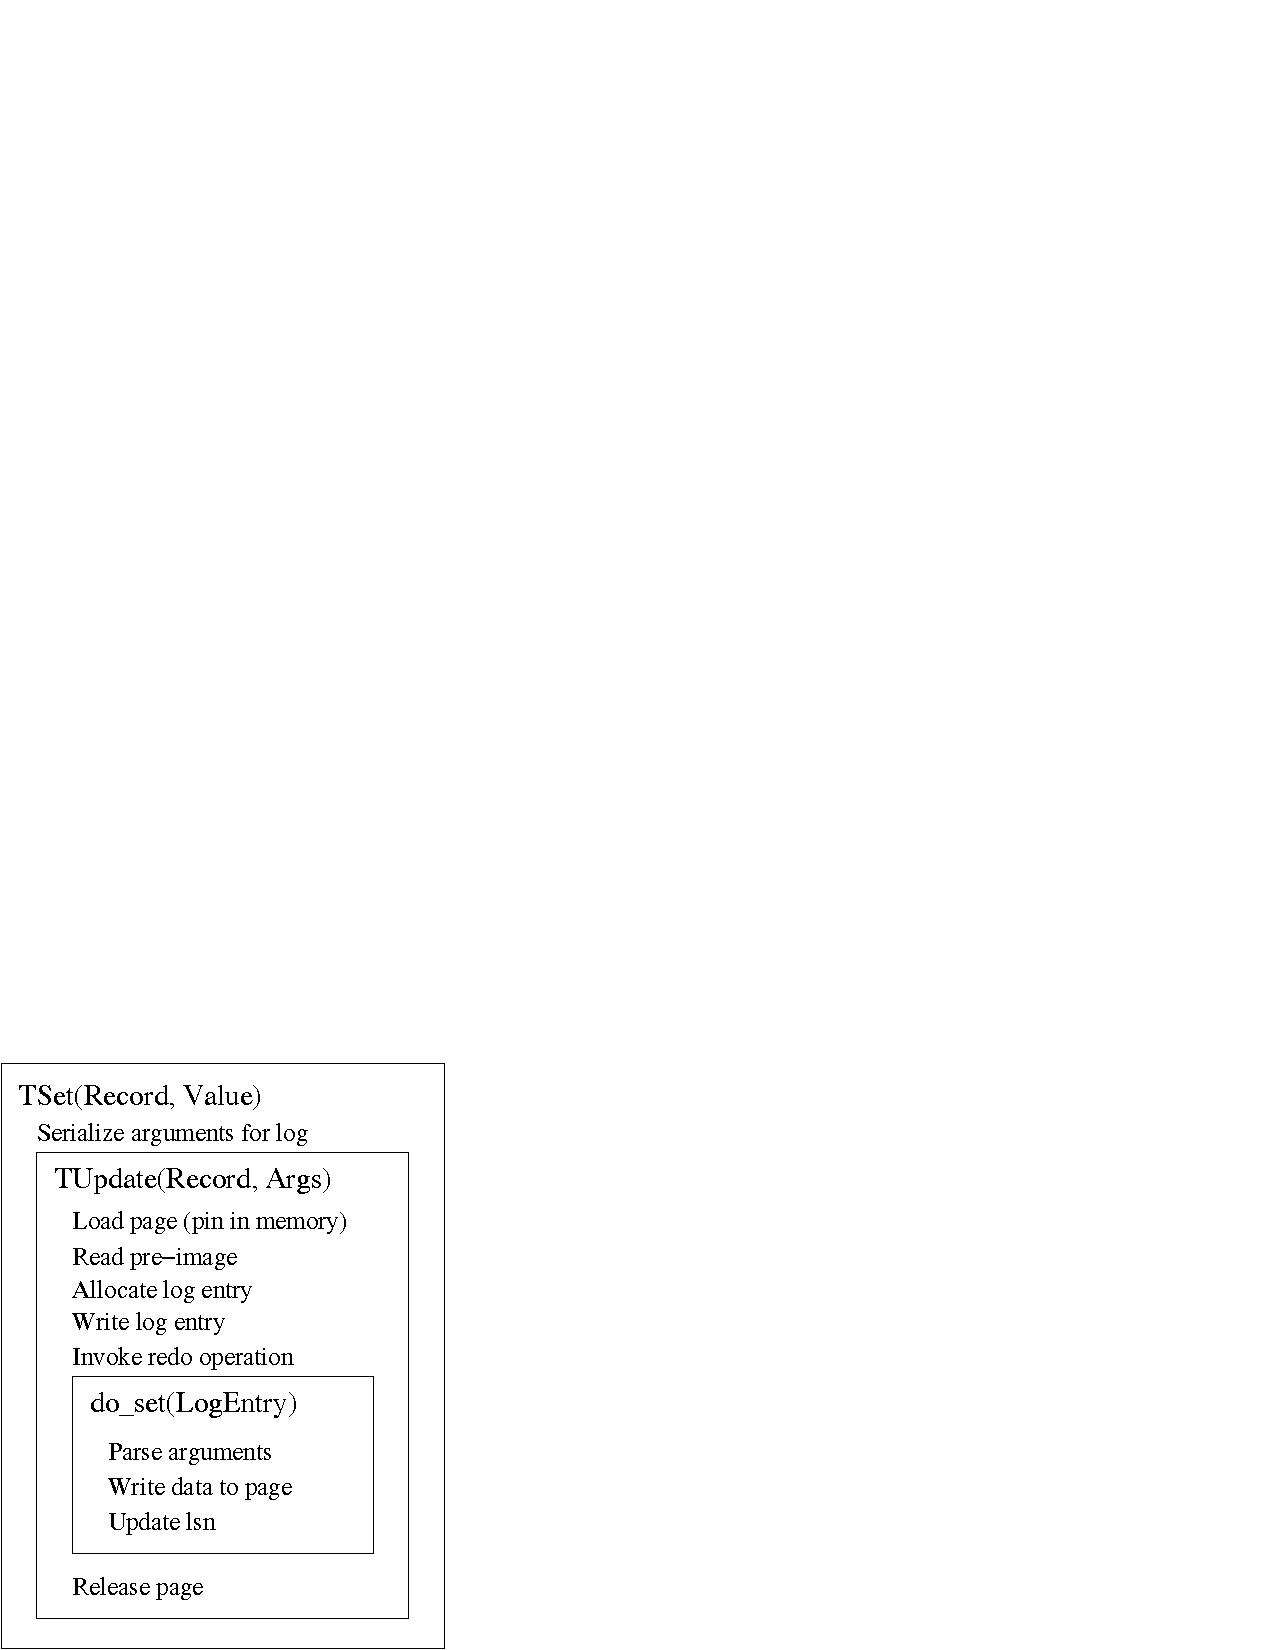
\includegraphics[%
  width=0.70\columnwidth]{TSetCall.pdf}


\caption{Runtime behavior of a simple operation. Tset() and do\_set() are
implemented as extensions, while Tupdate() is built in. New operations
need not be aware of the complexities of LLADD.}
\end{figure}


This way, the operation's behavior during recovery's redo phase (an
uncommon case) will be identical to the behavior during normal processing,
making it easier to spot bugs. Similarly, undo and redo operations take
an identical set of parameters, and undo during recovery is the same 
as undo during normal processing.  This makes recovery bugs more obvious and allows redo
functions to be reused to implement undo. 

Although any latches acquired by the wrapper function will not be
reacquired during recovery, the redo phase of the recovery process
is single threaded. Since latches acquired by the wrapper function
are held while the log entry and page are updated, the ordering of
the log entries and page updates associated with a particular latch
must be consistent. However, some care must be taken to ensure proper
undo behavior.


\subsubsection{Concurrency and Aborted Transactions}

Section \ref{sub:OperationProperties} states that LLADD does not
allow cascading aborts, implying that operation implementors must
protect transactions from any structural changes made to data structures
by uncomitted transactions, but LLADD does not provide any mechanisms
designed for long term locking. However, one of LLADD's goals is to
make it easy to implement custom data structures for use within safe,
multi-threaded transactions. Clearly, an additional mechanism is needed.

The solution is to allow portions of an operation to 'commit' before
the operation returns.%
\footnote{We considered the use of nested top actions, which LLADD could easily
support. However, we currently use the slightly simpler (and lighter-weight)
mechanism described here. If the need arises, we will add support
for nested top actions.%
} An operation's wrapper is just a normal function, and therefore may
generate multiple log entries. First, it writes an undo-only entry
to the log. This entry will cause the \emph{logical} inverse of the
current operation to be performed at recovery or abort, must be idempotent,
and must fail gracefully if applied to a version of the database that
does not contain the results of the current operation. Also, it must
behave correctly even if an arbitrary number of intervening operations
are performed on the data structure.

The remaining log entries are redo-only, and may perform structural
modifications to the data structure. They should not make any assumptions
about the consistency of the current version of the database. Finally,
any prefix of the sequence of the redo-only operations performed by
this operation must leave the database in a consistent state. The
$B^{LINK}$ tree {[}...{]} is an example of a B-Tree implementation
that behaves in this way, as is the linear hash table implementation
discussed in Section \ref{sub:Linear-Hash-Table}. 

Some of the logging constraints introduced in this section may seem
strange at this point, but are motivated by the recovery process.


\subsection{Recovery}


\subsubsection{ANALYSIS / REDO / UNDO}

Recovery in AIRES consists of three stages, analysis, redo and undo
. The first, analysis, is
partially implemented by LLADD, but will not be discussed in this
paper. The second, redo, ensures that each redo entry in the log 
will have been applied each page in the page file exactly once.
The third phase, undo rolls back any transactions that were active
when the crash occured, as though the application manually aborted
them with the {}``abort()'' call.
  
After the analysis phase, the on-disk version of the page file
is in the same state it was in when LLADD crashed. This means that
some subset of the page updates performed during normal operation
have made it to disk, and that the log contains full redo and undo
information for the version of each page present in the page file.%
\footnote{Although this discussion assumes that the entire log is present, the
ARIES algorithm supports log truncation, which allows us to discard
old portions of the log, bounding its size on disk.%
} However, we make no further assumptions regarding the order in which
pages were propogated to disk. Therefore, redo must assume that any
data structures, lookup tables, etc. that span more than a single
page are in an inconsistent state. Therefore, as the redo phase re-applies
 the information in the log to the page file, it must address all pages directly. 

Therefore, the redo information for each operation in the log
must contain the physical address (page number) of the information
that it modifies, and the portion of the operation executed by a single
log entry must only rely upon the contents of the page that the log
entry refers to. Since we assume that pages are propagated to disk
atomicly, the REDO phase may rely upon information contained within
a single page.

Once redo completes, some prefix of the runtime log that contains 
complete entries for all committed transactions has been applied 
to the database.  Therefore, we know that the page file is in
a physically consistent state (although it contains portions of the
results of uncomitted transactions). The final stage of recovery is
the undo phase, which simply aborts all uncomitted transactions. Since
the page file is physically consistent, the transactions are aborted
exactly as they would be during normal operation. 


\subsubsection{Physical, Logical and Phisiological Logging.}

The above discussion avoided the use of some terminology that is common
in the database literature and which should be presented here. {}``Physical
loggging'' is the practice of logging physical (byte level) upates
and the physical (page number) addresses that they are applied to. 

It is subtly different than {}``physiological logging,'' which is
what LLADD recommends for its redo records. In physiological logging,
the physical (page number) address is stored, but the byte offset
and the actual difference are stored implicitly in the parameters
of some function. When the parameters are applied to the function,
it will update the page in a way that preserves application semantics.
This allows for some convenient optimizations. For example, data within
a single page can be re-arranged at runtime to produce contiguous
regions of free space, or the parameters passed to the function may
be significantly smaller than the physical change made to the page. 

{}``Logical logging'' can only be used for undo entries in LLADD,
and is identical to physiological logging, except that it stores a
logical address (the key of a hash table, for instance) instead of
a physical address. This allows the location of data in the page file
to change, even if outstanding transactions may have to roll back
changes made to that data. Clearly, for LLADD to be able to apply
logical log entries, the page file must be physically consistent,
ruling out use of logical logging for redo operations.

LLADD supports all three types of logging, and allows developers to
register new operations, which is the key to its extensibility. After
discussing LLADD's architecture, we will revisit this topic with a
concrete example.


\subsection{Summary}

This section presented a relatively simple set of rules and patterns
that a developer must follow in order to implement a durable, transactional
and highly-concurrent data structure using LLADD:

\begin{itemize}
\item Pages should only be updated inside of a redo or undo function.
\item An update to a page should update the LSN. 
\item If the data read by the wrapper function must match the state of
the page that the redo function sees, then the wrapper should latch
the relevant data.
\item Redo operations should address pages by their physical offset,
while Undo operations should use a more permenant address (such as
index key) if the data may move between pages over time.
\item An undo operation must correctly update a data structure if any
prefix of its corresponding redo operations are applied to the
structure, and if any number of intervening operations are applied to
the structure.
\end{itemize}
Because undo and redo operations during normal operation and recovery
are similar, most bugs will be found with conventional testing
strategies.  It is difficult to verify the final property, although a
number of tools could be written to simulate various crash scenarios,
and check the behavior of operations under these scenarios.  

Note that the ARIES algorithm is extremely complex, and we have left
out most of the details needed to implement it correctly.\footnote{The original ARIES paper was around 70 pages, and the ARIES/IM paper, which covered index implementation is roughly the same length}
  Yet, we believe we have covered everything that a programmer needs to know in order to implement new data structures using the basic functionality that ARIES provides. This was possible due to the encapsulation
of the ARIES algorithm inside of LLADD, which is the feature that
most strongly differentiates LLADD from other, similar libraries.
We hope that this will increase the availability of transactional
data primatives to application developers.


\section{LLADD Architecture}

%
\begin{figure}
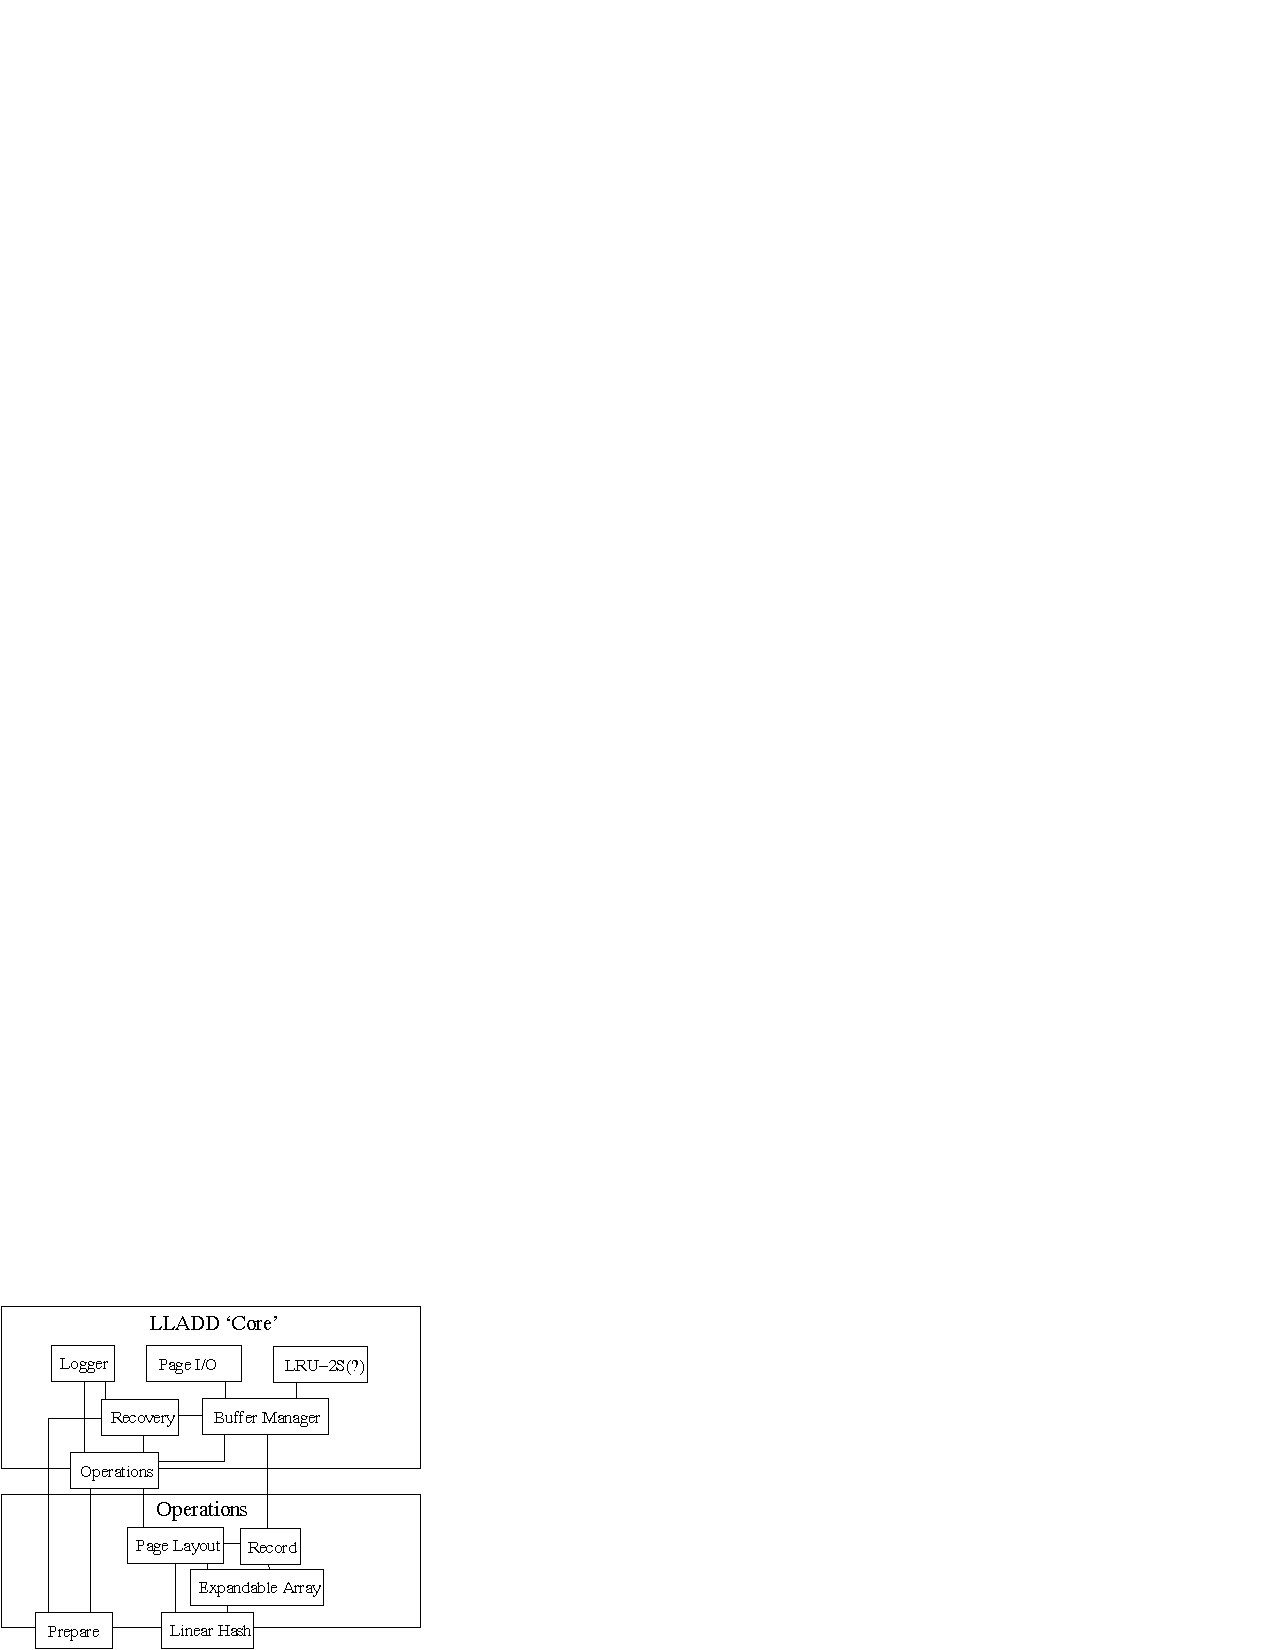
\includegraphics[%
  width=1.0\columnwidth]{LLADD-Arch2.pdf}


\caption{\label{cap:LLADD-Architecture}Simplified LLADD Architecture: The
core of the library places as few restrictions on the application's
data layout as possible. Custom {}``operations'' implement the client's
desired data layout. The seperation of these two sets of modules makes
it easy to improve and customize LLADD.}
\end{figure}
LLADD is a toolkit for building ARIES style transaction managers.
It provides user defined redo and undo behavior, and has an extendible
logging system with ... types of log entries so far. Most of these
extensions deal with data layout or modification, but some deal with
other aspects of LLADD, such as extensions to recovery semantics (Section
\ref{sub:Two-Phase-Commit}). LLADD comes with some default page layout
schemes, but allows its users to redefine this layout as is appropriate.
Currently LLADD imposes two requirements on page layouts. The first
32 bits must contain a log sequence number for recovery purposes,
and the second 32 bits must contain the page type.

While it ships with basic operations that support variable length
records, hash tables and other common data types, our goal is to
decouple all decisions regarding data format from the implementation
of the logging and recovery systems. Therefore, the preceeding section
is essentially documentation for potential users of the library, while
the purpose of the performance numbers in our evaluation section are
not to validate our hash table, but to show that the underlying architecture
is able to efficiently support interesting data structures.

Despite the complexity of the interactions between its modules, the
basic ARIES algorithm itself is quite simple. Therefore, in order to keep
LLADD simple, we started with a set of modules, and iteratively refined
the boundaries between these modules. A summary of the result is presented
in Figure \ref{cap:LLADD-Architecture}. The core of the LLADD library
is quite small at ... lines of code, and has been documented extensively.
We hope that we have exposed most of the subtle interactions between
internal modules in the online documentation. {[}... doxygen ...{]}

As LLADD has evolved, many of its sub-systems have been incrementally
improved, and we believe that the current set of modules is amenable
to the addition of new functionality. For instance, the logging module
interface encapsulates all of the details regarding its on disk format,
which would make it straightforward to implement more exotic logging
techniques such as using log shipping to maintain a 'warm replica'
for failover purposes, or the use of log replication to avoid physical
disk access at commit time. Similarly, the interface encodes the dependencies
between the logger and other subsystems, so, for instance, the requirements
that the buffer manager places on the logger would be obvious to someone
that attempted to alter the logging functionality.%
\footnote{The buffer manager must ensure that the logger has forced the appropriate
log entries to disk before writing a dirty page to disk. Otherwise,
it would be impossible to undo the changes that had been made to the
page.%
}

The buffer manager itself is another potential area for extension.
Because the interface between the buffer manager and LLADD is simple,
we would like to support transactional access to resources beyond
simple page files. Some examples include transactional updates of
multiple files on disk, transactional groups of program executions
or network requests, or even leveraging some of the advances being
made in the Linux and other modern operating system kernels. For example,
ReiserFS recently added support for atomic file system operations.
It is possible that this could be used to provide variable sized pages
to LLADD.  Combining some of these ideas should make it easy to 
implement some interesting applications.

From the testing point of view, the advantage of LLADD's division
into subsystems with simple interfaces is obvious. We are able to
use standard unit-testing techniques to test each of LLADD's subsystems
independently, and have documented both external and internal interfaces,
making it easy to add new tests and debug old ones. Furthermore, by
adding a 'simulate crash' operation to a few of the key components,
we can simulate application level crashes by clearing LLADD's internal
state, re-initializing the library and verifying that recovery was
successful. These tests currently cover approximately 90\% of the
code. We have not yet developed a mechanism that will allow us to
accurately model hardware failures, which is an area where futher
work is needed.  However, the basis for this work will be the development
of test harnesses that verify operation behavior in exceptional circumstances.

LLADD's performance requirements vary wildly depending on the workload
with which it is presented. Its performance on a large number of small,
sequential transactions will always be limited by the amount time
required to flush a page to disk. To some extent, compact logical
and physiological log entries improve this situation. On the other
hand, long running transactions only rarely force-write to disk and
become CPU bound. Standard profiling techniques of the overall library's
performance and microbenchmarks of crucial modules handle such situations
nicely. 

A more interesting set of performance requirements are imposed by
multithreaded workloads. Each module of LLADD is reentrant, and a
C preprocessor directive allows the entire library to be instrumented
in order to profile latching behavior, which is useful both for perfomance
tuning and for debugging purposes. A thread that is not involved in
an I/O request never needs to wait for a latch held by a thread that
is waiting for I/O.%
\footnote{Strictly speaking, this statement is only true for the LLADD's core.
However, there are variants of most popular data structures that allow
us to preserve these invariants. LLADD can correctly support operations
whether or not they have these properties.%
}

There are a number of performance optimizations that are specific
to multithreaded operations that we do not perform. The most glaring
omission is log bundling; if multiple transactions commit at once,
LLADD must force the log to disk one time per transaction. This problem
is not fundamental, but simply has not made it into the current code
base. Similarly, since page eviction requires a force-write if the
full ARIES recovery algorithm is in use, we could implement a thread
that asynchronously maintained a set of free buffer pages. We plan to 
implement such optimizations, but they are not reflected
in this paper's performance figures.


\section{Sample Operations}

In order to validate LLADD's architecture, and to show that it simplifies
the creation of efficient data structures, we have have implemented
a number of simple extensions. In this section, we describe their
design, and provide some concrete examples of our experiences extending
LLADD.


\subsection{Linear Hash Table\label{sub:Linear-Hash-Table}}

Linear hash tables are hash tables that are able to extend their bucket
list incrementally at runtime. They work as follows. Imagine that
we want to double the size of a hash table of size $2^{n}$, and that
the hash table has been constructed with some hash function $h_{n}(x)=h(x)\, mod\,2^{n}$
Choose $h_{n+1}(x)=h(x)\, mod\,2^{n+1}$ as the hash function for
the new table. Conceptually we are simply prepending a random bit
to the old value of the hash function, so all lower order bits remain
the same. At this point, we could simply block all concurrent access
and iterate over the entire hash table, reinserting values according
to the new hash function. 

However, because of the way we chose $h_{n+1}(x),$ we know that the
contents of each bucket, $m$, will be split betwen bucket $m$ and
bucket $m+2^{n}$. Therefore, if we keep track of the last bucket
that was split, we can split a few buckets at a time, resizing the
hash table without introducing long pauses while we reorganize the
hash table.{[}...{]} We can handle overflow using standard techniques.
LLADD's linear hash table uses linked lists of overflow buckets.

For this scheme to work, we must be able to address a portion of the
page file as though it were an expandable array. We have implemented
this functionality as a seperate module, but will not discuss it here.

For the purposes of comparison, we provide two linear hash implementations.
The first is straightforward, and is layered on top of LLADD's standard
record setting operation, Tset(), and therefore performs physical
undo. This implementation provided a stepping stone to the more sophisticated
version which employs logical undo, and uses an identical on-disk
layout. As we discussed earlier, logical undo provides more opportunities
for concurrency, while decreasing the size of log entries. In fact,
the physical-undo implementation of the linear hash table cannot support
concurrent transactions, while threads utilizing the physical-undo 
implementation never hold locks on more than two buckets.%
\footnote{However, only one thread may expand the hashtable at once.  In order to amortize the overhead of initiating an expansion, and to allow concurrent insertions, the hash table is expanded in increments of a few thousand buckets.}%
\begin{figure}
~~~~~~~~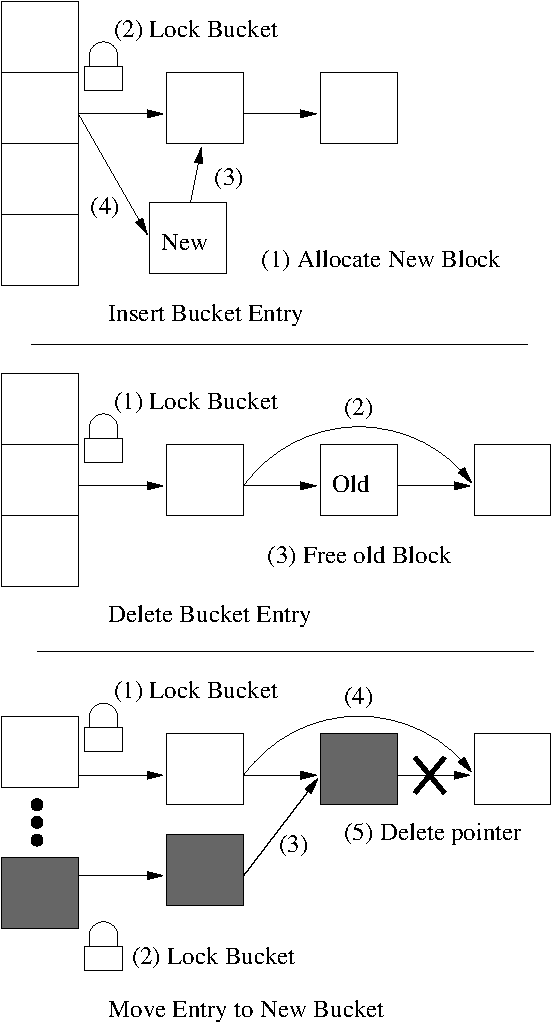
\includegraphics[%
  width=0.80\columnwidth]{LinkedList.pdf}


\caption{\label{cap:Linear-Hash-Table}Linear Hash Table Bucket operations.}
\end{figure}


Because another module provides the resizable arrays needed for the
bucket list, the complexity of the linear hash algorithm is in two
areas. The first, linked list management, is straightforward in the
physical case, but must be performed in a specific order in the logical
case. See Figure \ref{cap:Linear-Hash-Table} for a sequence of steps
that safely implement the necessary linked list operations. Note that
in the first two cases, the portion of the linked list that is visible
from LLADD's point of view is always consistent. This is important
for crash recovery; it is possible that LLADD will crash before the
entire sequence of operations has been completed. The logging protocol
guarantees that some prefix of the log will be available. Therefore,
as long as the run-time version of the hash table is always consistent,
we do not have to consider the impact of skipped updates, but we must
be certain that the logical consistency of the linked list is maintained
at all steps. Here, the challenge comes from the fact that the buffer
manager only provides atomic updates of single pages; in practice,
a linked list may span pages.

The last case, where buckets are split as the bucket list is expanded,
is a bit more complicated. We must maintain consistency between two
linked lists, and a page at the begining of the hash table that contains
the last bucket that we successfully split. Here, we misuse the undo
entry to ensure proper crash recovery. Our bucket split algorithm
is idempotent, so it may be applied an arbitrary number of times to
a given bucket with no ill-effects. Also note that (for our purposes),
there is never a good reason to undo a bucket split, so we can safely
apply the split whether or not the current transaction commits.

First, an 'undo' record that checks the hash table's meta data and
redoes the split if necessary is written (this record has no effect 
unless we crash during this bucket split). Second, we write (and execute) a series
of redo-only records to the log. These encode the bucket split, and follow
the linked list protocols listed above. Finally, we write a redo-only
entry that updates the hash table's metadata.%
\footnote{Had we been using nested top actions, we would not need the special
undo entry, but we would need to store physical undo information for
each of the modifications made to the bucket. This method does have
the disadvantage of producing a few redo-only entries during recovery,
but recovery is an uncommon case, and the number of such entries is
bounded by the number of entries that would be produced during normal 
operation.%
}

We allow pointer aliasing at this step so that a given key can be
present for a short period of time in both buckets. If we crash before
the undo entry is written, no harm is done. If we crash after the
entire update makes it to log, the redo stage will set the hash's
metadata appropriately, and the 'undo' record becomes a no-op. If
we crash in the middle of the bucket split, we know that the current
transaction did not commit, and that recovery will execute the 'undo'
record. It will see that the bucket split is still pending and finish
splitting the bucket appropriately. Since the bucket split is idempotent,
and we've arranged for it to behave correctly regardless of the point
at which it was interrupted, the hastable is correctly restored. 

Note that there is a point during the undo phase where the bucket
is in an inconsistent physical state, although normally the redo phase
is able to bring the database to a fully consistent physical state.
We handle this by obtaining a runtime lock on the bucket during normal
operation. This runtime lock blocks any attempt to write log entries
that alter a bucket that is being split, so we know that no other
logical operations will attempt to access an inconsistent bucket.

Since the second implementation of the linear hash table uses logical
undo, we are able to allow concurrent updates to different portions
of the table. This is not true in the case of the implementation that
uses pure physical logging, as physical undo cannot generally tolerate
concurrent structural modifications to data structures.


\subsection{Two Phase Commit\label{sub:Two-Phase-Commit}}

The two phase commit protocol is used in clustering applications where
multiple, well maintained, well connected computers must agree upon
a set of successful transactions. Some of the systems could crash,
or the network could fail during operation, but we assume that such
failures are temporary. Two phase commit designates a single computer
as the coordinator of a given transaction. This computer contacts
the other systems participating in the transaction, and asks them
to prepare to commit the transaction. If a subordinate system sees
that an error has occurred, or the transaction should be aborted for
some other reason, then it informs the coordinator. Otherwise, it
enters the \emph{prepared} state, and tells the coordinator that it
is ready to commit. At some point in the future, the coordinator will
reply telling the subordinate to commit or abort. From LLADD's point
of view, the interesting portion of this algorithm is the \emph{prepared}
state, since it must be able to commit a prepared transaction if it
crashes before the coordinator responds, but cannot commit before
hearing the response, since it may be asked to abort the transaction.

Implementing the prepare state on top of the ARIES algorithm constists
of writing a special log entry that informs the undo portion of the
recovery phase that it should stop rolling back the current transaction
and instead add it to the list of active transactions.%
\footnote{Also, any locks that the transaction obtained should be restored,
which is outside of the scope of LLADD, although this functionality
could be added relatively easily if a lock manager were implemented
on top of LLADD.%
} Due to LLADD's extendible logging system, and the simplicity
of its recovery code, it took an afternoon to add a prepare operation
to LLADD.


\section{Evaluation}

We hope that the preceeding sections have given the reader an idea
of the usefulness and extensibility of the LLADD library. In this
section we focus on performance evaluation.

In order to evaluate the physical and logical hashtable implementations,
we first ran a test that inserts some tuples into the database. For
this test, we chose fixed length key, values pairs of integers. For
simplicity, our hashtable implementations currently only support fixed-length
keys and values, so this this test puts us at a significant advantage.
It also provides an example of the type of workload that LLADD handles
well, since LLADD is specifically designed to support application
specific transactional data structures. 

%
\begin{figure*}
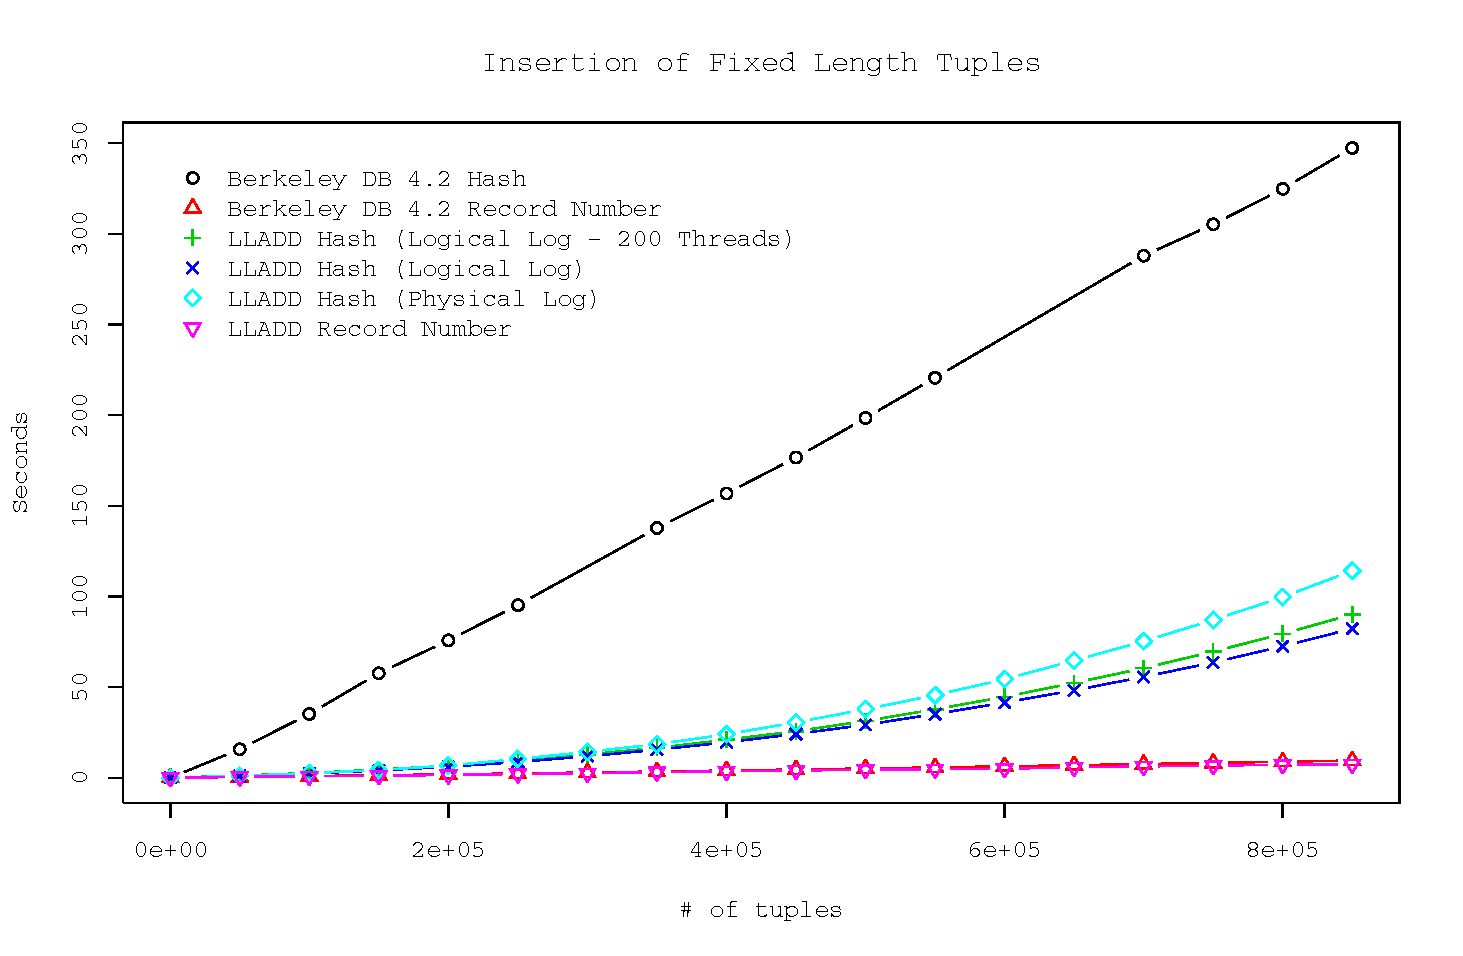
\includegraphics[%
  width=1.0\textwidth]{INSERT.pdf}


\caption{\label{cap:INSERTS}The final data points for LLADD's and Berkeley
DB's record number based storage are 7.4 and 9.5 seconds, respectively.
LLADD's hash table is significantly faster than Berkeley DB in this
test, but provides less functionality than the Berkeley DB hash. Finally,
the logical logging version of LLADD's hash table is faster than the
physical version, and handles the multi-threaded test well. The threaded
test split its workload into 200 seperate transactions.}
\end{figure*}
The times included in Figure \ref{cap:INSERTS} include page file
and log creation, insertion of the tuples as a single transaction,
and a clean program shutdown. We used the 'transapp.cs' program from
the Berkeley DB 4.2 tutorial to run the Berkeley DB tests, and hardcoded
it to use integers instead of strings. We used the Berkeley DB {}``DB\_HASH''
index type for the hashtable implementation, and {}``DB\_RECNO''
in order to run the {}``Record Number'' test.

Since LLADD addresses records as \{Page, Slot, Size\} triples, which
is a lower level interface than Berkeley DB exports, we used the expandible
array that supports the hashtable implementation to run the {}``LLADD
Record Number'' test.

One should not look at Figure \ref{cap:INSERTS}, and conclude {}``LLADD
is almost five times faster than Berkeley DB,'' since we chose a
hash table implementation that is tuned for fixed-length data. Instead,
the conclusions we draw from this test are that, first, LLADD's primative
operations are on par, perforance wise, with Berkeley DB's, which
we find very encouraging. Second, even a highly tuned implementation
of a 'simple,' general purpose data structure is not without overhead,
and for applications where performance is important a special purpose
structure may be appropriate.

As a final note on our performance graph, we would like to address
the fact that LLADD's hashtable curve is non-linear. LLADD currently
uses a fixed-size in-memory hashtable implementation in many areas,
and it is possible that we exceed the fixed-size of this hashtable
on the larger test sets. Also, LLADD's buffer manager is currently
fixed size. Regardless of the cause of this non-linearity, we do not
believe that it is fundamental to our implementation.

{[} 

Still need to run the multi-threaded tests. The physical one's performance
should strictly degrade as the number of threads increases, while
the logical one's performance should increase for a while, and then
begin to degrade. Hopefully the logical one's peak performance will
be better than the physical implementation's peak performance.

I still haven't decided how to run the 2PC performance numbers. Maybe
I could run a speed-up or scale-up test on it.

I expect this section to be two pages, including graphs.

{]}


\section{Future Work}

LLADD is an extendible implementation of the ARIES algorithm. This
allows application developers to incorporate transactional recovery
into a wide range of systems. We have a few ideas along these lines,
and also have some ideas for extensions to LLADD itself.

LLADD currently relies upon its buffer manager for page oriented storage.
Although we did not have space to discuss it in this paper, we have
a blob implementation that stores large data outside of the page file.
This concept could be extended to arbitrary primatives, such as transactional
updates to file system directory trees, integration of networking,
or other operations directly into LLADD transactions. Doing this would
allow LLADD to act as a sort of 'glue-code' between various systems,
ensuring data integrity and adding database-style functionality, such
as continuous backup to systems that currently do not provide such
mechanisms. We believe that there is quite a bit of room for the developement
of new software systems in the space between the high-level, but sometimes
inappropriate interfaces exported by database servers, and the low-level,
general purpose primatives supported by current file systems.

Currently, while we have implemented a two phase commit algorithm,
LLADD really is not very network aware. If we provided a clean abstraction
that allowed LLADD extensions and operations to cross network boundaries,
then we could provide a wider range of network consistency algorithms,
and cleanly support the implementation of operations that perform
well in networked and in local environments.

While LLADD is re-entrant, its latching mechanisms only provide physical
consistency. Traditionally, lock-managers, which provide higher levels
of consistency have been tightly coupled with transactional page implementations.
Generally, the semantics of undo and redo operations provided by the
transactional page layer and its associated data structures determine
the level of concurrency that is possible. Since prior systems provide
a set of primitives to their users, these systems encapsulated the
interactions between the lock manager, on-disk formats and the transactional
page layer. Finally, at recovery time it is often desirable to reacquire
locks on behalf of a transaction. Without extensible logging and without
modifying the recovery code, it is impossible to ensure that such
locks are correctly restored. By providing extensible logging, data-structures,
and undo/redo semantics, LLADD removes these reasons for coupling
the lock manager and the rest of the storage mechanisms. The flexiblity
offered by splitting the lock manager and the ARIES algorithm into
independent sub-systems, and allowing users to independently extend
either module seems to outweigh the extra complexity that will be
added to LLADD's interface. In particular, most difficulties related
to locking seem to be data-structure dependent, suggesting that, like
page layout or the semantics of various types of log entires, they
are largely orthagonal to the atomicity and durability algorithms
implemented by LLADD.

By releasing LLADD to the community, we hope that we will be able
to provide a toolkit that aids in the development of real-world applications,
and is flexible enough for use as a research platform.


\section{Conclusion}

\section{Acknowledgements}

\section{Availability}

LLADD is free software, available at:

\begin{center}
{\tt http://www.sourceforge.net/projects/lladd}\\
\end{center}

\begin{thebibliography}{99}

\bibitem[Beazley]{beazley} D.~M.~Beazley and P.~S.~Lomdahl, 
{\em Message-Passing Multi-Cell Molecular Dynamics on the Connection
Machine 5}, Parall.~Comp.~ 20 (1994) p. 173-195.

\bibitem[RealName]{CitePetName} A.~N.~Author and A.~N.~Other, 
{\em Title of Riveting Article}, JournalName VolNum (Year) p. Start-End

\bibitem[ET]{embed} Embedded Tk, \\
{\tt ftp://ftp.vnet.net/pub/users/drh/ET.html}

\bibitem[Expect]{expect} Don Libes, {\em Exploring Expect}, O'Reilly \& Associates, Inc. (1995).

\bibitem[Heidrich]{heidrich} Wolfgang Heidrich and Philipp Slusallek, {\em
Automatic Generation of Tcl Bindings for C and C++ Libraries.},
USENIX 3rd Annual Tcl/Tk Workshop (1995).

\bibitem[Ousterhout]{ousterhout} John K. Ousterhout, {\em Tcl and the Tk Toolkit}, Addison-Wesley Publishers (1994).

\bibitem[Perl5]{perl5} Perl5 Programmers reference,\\
{\tt http://www.metronet.com/perlinfo/doc}, (1996).

\bibitem[Wetherall]{otcl} D. Wetherall, C. J. Lindblad, ``Extending Tcl for
Dynamic Object-Oriented Programming'', Proceedings of the USENIX 3rd Annual Tcl/Tk Workshop (1995).

\end{thebibliography}


\end{document}
